%%
%% This is file `example.tex',
%% generated with the docstrip utility.
%%
%% The original source files were:
%%
%% coppe.dtx  (with options: `example')
%% 
%% This is a sample monograph which illustrates the use of `coppe' document
%% class and `coppe-unsrt' BibTeX style.
%% 
%% \CheckSum{1416}
%% \CharacterTable
%%  {Upper-case    \A\B\C\D\E\F\G\H\I\J\K\L\M\N\O\P\Q\R\S\T\U\V\W\X\Y\Z
%%   Lower-case    \a\b\c\d\e\f\g\h\i\j\k\l\m\n\o\p\q\r\s\t\u\v\w\x\y\z
%%   Digits        \0\1\2\3\4\5\6\7\8\9
%%   Exclamation   \!     Double quote  \"     Hash (number) \#
%%   Dollar        \$     Percent       \%     Ampersand     \&
%%   Acute accent  \'     Left paren    \(     Right paren   \)
%%   Asterisk      \*     Plus          \+     Comma         \,
%%   Minus         \-     Point         \.     Solidus       \/
%%   Colon         \:     Semicolon     \;     Less than     \<
%%   Equals        \=     Greater than  \>     Question mark \?
%%   Commercial at \@     Left bracket  \[     Backslash     \\
%%   Right bracket \]     Circumflex    \^     Underscore    \_
%%   Grave accent  \`     Left brace    \{     Vertical bar  \|
%%   Right brace   \}     Tilde         \~}
%%
\documentclass[grad,numbers]{coppe}
\usepackage{amsmath,amssymb}
\usepackage{hyperref}
\usepackage[utf8]{inputenc}
\usepackage[brazil]{babel}
\usepackage[T1]{fontenc}
\usepackage{graphicx}
\usepackage{placeins}

\makelosymbols
\makeloabbreviations

\begin{document}
  \title{PIPA Bot: uma solução chatbot para o projeto PIPA UFRJ}
  \foreigntitle{PIPA Bot: a chatbot solution for PIPA UFRJ project}
  \author{Lucas Santos}{de Paula}
  \advisor{Prof.}{Guilherme Horta}{Travassos}{D.Sc.}
  \advisor{Prof.}{Taísa Guidini}{Gonçalves}{Ph.D.}
  %\advisor{Prof.}{Nome do Terceiro Orientador}{Sobrenome}{D.Sc.}

  \examiner{Prof.}{Nome do Primeiro Examinador Sobrenome}{D.Sc.}
  \examiner{Prof.}{Nome do Segundo Examinador Sobrenome}{Ph.D.}
  \examiner{Prof.}{Nome do Terceiro Examinador Sobrenome}{D.Sc.}
  \examiner{Prof.}{Nome do Quarto Examinador Sobrenome}{Ph.D.}
  \examiner{Prof.}{Nome do Quinto Examinador Sobrenome}{Ph.D.}
  
  
  
  \department{ECI}% Confira a tabela a seguir para saber como preencher o comando \department de acordo com seu curso (Graduação - Poli) ou programa (Pós-Graduação - COPPE).
  
  %%%%%% Para alunos da POLI %%%%%%
  
  %% Course											Option
  %% Engenharia Ambiental                             EA
  %% Engenharia Civil                                 ECV
  %% Engenharia de Computação e Informação            ECI
  %% Engenharia de Controle e Automação               ECA
  %% Engenharia de Materiais                          EMAT
  %% Engenharia de Petróleo                           EPT
  %% Engenharia de Produção                           EPR
  %% Engenharia Eletrônica e de Computação            EEC
  %% Engenharia Elétrica                              EET
  %% Engenharia Mecânica                              EMC
  %% Engenharia Metalúrgica                           EMET
  %% Engenharia Naval e Oceânica                      ENO
  %% Engenharia Nuclear                               ENU
  
  
  %%%%%% Para alunos da COPPE %%%%%%
  
  %% Program											Option
  %% Engenharia Biomédica								PEB
  %% Engenharia Civil									PEC
  %% Engenharia Elétrica								PEE
  %% Engenharia Mecânica								PEM
  %% Engenharia Metalúrgica e de Materiais				PEMM
  %% Engenharia Nuclear									PEN
  %% Engenharia Oceânica								PENO
  %% Planejamento Energético							PPE
  %% Engenharia de Produção								PEP
  %% Engenharia Química									PEQ
  %% Engenharia de Sistemas e Computação				PESC
  %% Engenharia de Transportes							PET
  
  
  
  
  
  
  \date{08}{2019}

  \keyword{Chatbot}
  \keyword{Lean Inception}
  \keyword{Engenharia de Software}

  \maketitle

  \frontmatter
  
  \makecatalog
  
  \dedication{A Paulo Cardoso, Hercília Cardoso e Maria Alves (in memoriam).}

  \chapter*{Agradecimentos}

  Gostaria de agradecer a todos.

  \begin{abstract}

  \textit{Chatbots} são sistemas de software que fazem uso de processamento de linguagem natural para estabelecer diálogos com pessoas como se fossem humanos. Podem atuar como um canal facilitador para a comunicação entre humanos e entidades como empresas, projetos sociais e de pesquisa, hospitais, etc. Esse trabalho apresenta o desenvolvimento do PipaBot, o \textit{chatbot} do Projeto Infância e Poluentes Ambientais (PIPA-UFRJ), que deverá atender cerca de duas mil mães participantes.
  
  O PipaBot foi desenvolvido em duas plataformas: através do aplicativo Messenger do Facebook e também no \textit{website} do PIPA. Através dele é possível obter informações sobre o projeto e seus objetivos, e também realizar uma identificação como paciente do projeto, que libera acesso a informações como consultas e resultados de exames médicos.
  
  A PipaBot foi validado segundo o modelo de aceitação da tecnologia (TAM - \textit{Tecnological Acceptance Model}), com a avaliação de 13 usuários sendo dividos em dois grupos principais: profissionais da saúde (pesquisadores do projeto PIPA-UFRJ), e profissionais de computação (pesquisadores da COPPE-UFRJ) tendo resultados satisfatórios os quais serão apresentados com mais detalhes neste trabalho.
  \end{abstract}

  \begin{foreignabstract}

  In this work, we present ...

  \end{foreignabstract}

  \tableofcontents
  \listoffigures
  \listoftables
  \printlosymbols
  \printloabbreviations

  \mainmatter
%  \doublespacing
  
    \chapter{Introdução}
  
  \section{Tema}
  
  O tema do trabalho é o desenvolvimento de um dispositivo que realize a medição da frequência respiratória dentro de uma faixa sensível para respostas psicofisiológicas. Este dispositivo deve possibilitar o monitoramento e a extração de dados que auxiliarão em estudos os quais correlacionam alguns parâmetros da frequência respiratória com funções psicofisiológicas, como aquelas observadas sob alterações cognitivas, emocionais, sob estresse  doenças mentais.
  
  \section{Delimitação}
  
  O objeto de estudo é o desenvolvimento de um protótipo capaz de mensurar comportamentos respiratórios tais quais a frequência de inspiração e expiração, para, a partir desse, analisar a viabilidade de desenvolvimento de um equipamento com baixo custo voltado ao uso científico. As medições terão como finalidade a obtenção de dados, referentes à frequência respiratória do paciente, a serem utilizados em experimentos que vinculem comportamentos saudáveis e suas variantes clínicas à respiração humana. O estudo, limita-se à obtenção desses dados, não abrangendo, a priori, interpretações acerca das correlações obtidas em eventuais medições realizadas, além de possuir, em princípio, finalidade meramente científica, sem conter qualquer estudo sobre viabilidade comercial de produtos que venham a ser desenvolvidos.
  
  \section{Justificativa}
 
   Segundo Sebastião Gusmão \cite{gusmao2004historia}, a medicina como ciência, baseada na interpretação natural da doença e não em magia e empirismo, como ocorria na medicina arcaica, tem sua origem no século V a.C com Hipócrates (c. 460-375 a.C). Desde então, análises e estudos sobre o funcionamento do corpo humano, bem como as interações deste com o meio ambiente, vêm sendo realizados em constante evolução. Hoje, sabe-se que o organismo humano é composto de diversas partes que, em conjunto, garantem o seu funcionamento adequado. O corpo é, portanto, um sistema complexo no qual atuam diversas variáveis. Sendo assim, grande parte dos estudos científicos atuais voltam seus métodos e análises ao estudo dos parâmetros que possuem influências para o bom ou mal funcionamento do organismo. Atualmente, sabe-se que diversas doenças psicofisiológicas produzem variações no funcionamento normal do corpo, como alterações na produção de determinados hormônios, no batimento cardíaco, na pressão arterial ou na concentração de $CO_2$ no sangue. 
   
   Estudos recentes demonstram que é possível por exemplo, induzir pânico em ratos apenas alterando a concentração de $O_2$ ou de $CO_2$ do ar por eles respirado \cite{spiacci2015serotonin} \cite{spiacci2018panic}. A respiração humana é, assim como nos ratos, o processo natural responsável pela troca do $CO_2$ com o $O_2$.    
    
   Ao realizar uma análise de correspondência (correlação, regressão, inferência etc.) entre determinado comportamento biológico e algum quadro clínico específico, o 		pesquisador necessita realizar, de alguma maneira, a mensuração das variáveis que compõem o comportamento com acurácia e significado preditivo para a sensibilidade e a especificidade dos resultados. Nesse sentido, o desenvolvimento de um equipamento de baixo custo capaz de coletar dados referentes ao comportamento respiratório torna-se parte essencial à evolução do estudo científico. 
      
   Munido dessa motivação, neste trabalho, apresentam-se estudos para viabilidade do desenvolvimento de uma tecnologia com baixo custo capaz de monitorar o comportamento do fluxo respiratório de pacientes, servindo então como base para estudos científicos na área de neurociência comportamental. 
 
  \section{Objetivos}
  
	O objetivo geral deste estudo é, então, desenvolver um protótipo de equipamento capaz de realizar a aquisição de dados referentes à frequência respiratória em humanos, incluindo parâmetros que possam ser utilizados em pesquisas neurocientíficas. Desta forma, tem-se como objetivos específicos: (1) Realizar a mensuração da frequência respiratória (2) desenvolver os métodos de medida da frequência respiratória para extrair suas variantes no domínio do tempo e da frequência; e (3) Possibilitar a exportação dos dados para análises futuras.
  
  
  \section{Metodologia}

	A priori, a medição da frequência respiratória seria obtida indiretamente pela variação da temperatura do ar próximo à narina do paciente, uma vez que, em um ambiente controlado, o ar inalado possui uma temperatura inferior à do ar exalado. Contudo, no decorrer do desenvolvimento, foi observado que seria inviável a realização desse tipo de medição devido à baixa variação entre essas duas temperaturas e à velocidade de resposta necessária para a obtenção dos dados de forma confiável utilizando equipamentos de baixo custo. Para contornar esse problema, foi utilizada a propriedade de autoaquecimento do termistor, que passou a ser utilizado como um sensor de fluxo. Ou seja, o sistema não mais tenta inferir a frequência respiratória com base no aumento da temperatura ambiente ocasionada pela saída de ar quente do corpo humano, ao contrário, ele aplica uma corrente muito alta no sensor forçando-o a atingir por conta própria uma temperatura ainda maior em seu estado permanente e, no momento de seu encontro com qualquer fluxo de ar resultante da respiração humana, o sensor registra uma alta queda de temperatura, registrando, de forma mais nítida o momento da ação respiratória.

	O termistor é um resistor variável à temperatura, escolhido principalmente por suas propriedades de autoaquecimento e pela variação exponencial de sua resistência em relação à mudança na temperatura, contrário a grande parte dos demais sensores que possuem uma relação linear entre essas variáveis. Trabalhar com um sensor de cuja curva característica é exponencial facilita detecções de pequenas variações na temperatura, gerando grandes mudanças na resistência, em contrapartida, adiciona complexidade ao sistema dado que trabalhar com relações lineares é, em geral, mais simples. A escolha do termistor é portanto perfeita porque sua contrapartida sequer implica em complicações para o sistema deste trabalho, dado que, em princípio, não interessa uma medição precisa da temperatura, mas sim o registro dos eventos de inspiração e expiração.
	
	O sistema é composto de uma fonte capaz de entregar ao sensor corrente suficiente para que este entre em estado de autoaquecimento e atinja uma temperatura alta o suficiente para se tornar sensível à variação provocada pelos fluxos de ar, um circuito regulador responsável por filtrar sinais indesejados e controlar a corrente de entrada no termistor, um microcontrolador que irá realizar as medições e um software capaz de exportar os dados para que esses possam ser tratados e estudados em suas aplicações.  

  \section{Organização do Trabalho}
  Nos próximos capítulos serão apresentados em mais detalhes as aplicações, o desenvolvimento e os resultados obtidos com esse trabalho, organizados da seguinte forma:
  
  O capítulo 2 apresentará a motivação para o desenvolvimento do equipamento, as aplicações no campo da medicina e um resumo do funcionamento fisiológico da respiração humana. 
  
  O capítulo 3 tratará sobre desenvolvimento do sistema, hardware e software bem como o raciocínio por trás da arquitetura.
  
  O capítulo 4 apresentará a lista de materiais utilizados no projeto
  
  O capítulo 5 será destinado à conclusão desse projeto, com o protótipo construído no último ciclo de desenvolvimento, limitações encontradas ao longo das etapas e também possíveis melhorias para trabalhos futuros.
 

    \chapter{Revisão da Literatura}
  
  \section{NLP - Processamento de Linguagem Natural}
  O processamento de linguagem natural é uma vertente específica da Inteligência Artificial que utiliza conhecimentos da língua e de comunicação para melhorar a interação homem-máquina. É possível sintetizar o conceito de NLP como "a habilidade de um computador em processar a mesma linguagem que os humanos usam no cotidiano\cite{chatbot_definition}. Linguística, semântica, teoria da comunicação e processamento de sinais são algumas das áreas que auxiliam no processamento de linguagem natural.
  
  Um sistema conversacional é capaz de detectar \textit{intents} e \textit{entities}. O intent é o objetivo ou propósito da interação do usuário com o chatbot, enquanto uma entity é uma caraterística que adiciona valor a um intent\cite{jain2018convey} como demonstradona figura \ref{fig:nlp}.
  
  \begin{figure}[h!]
  	\begin{center}
  		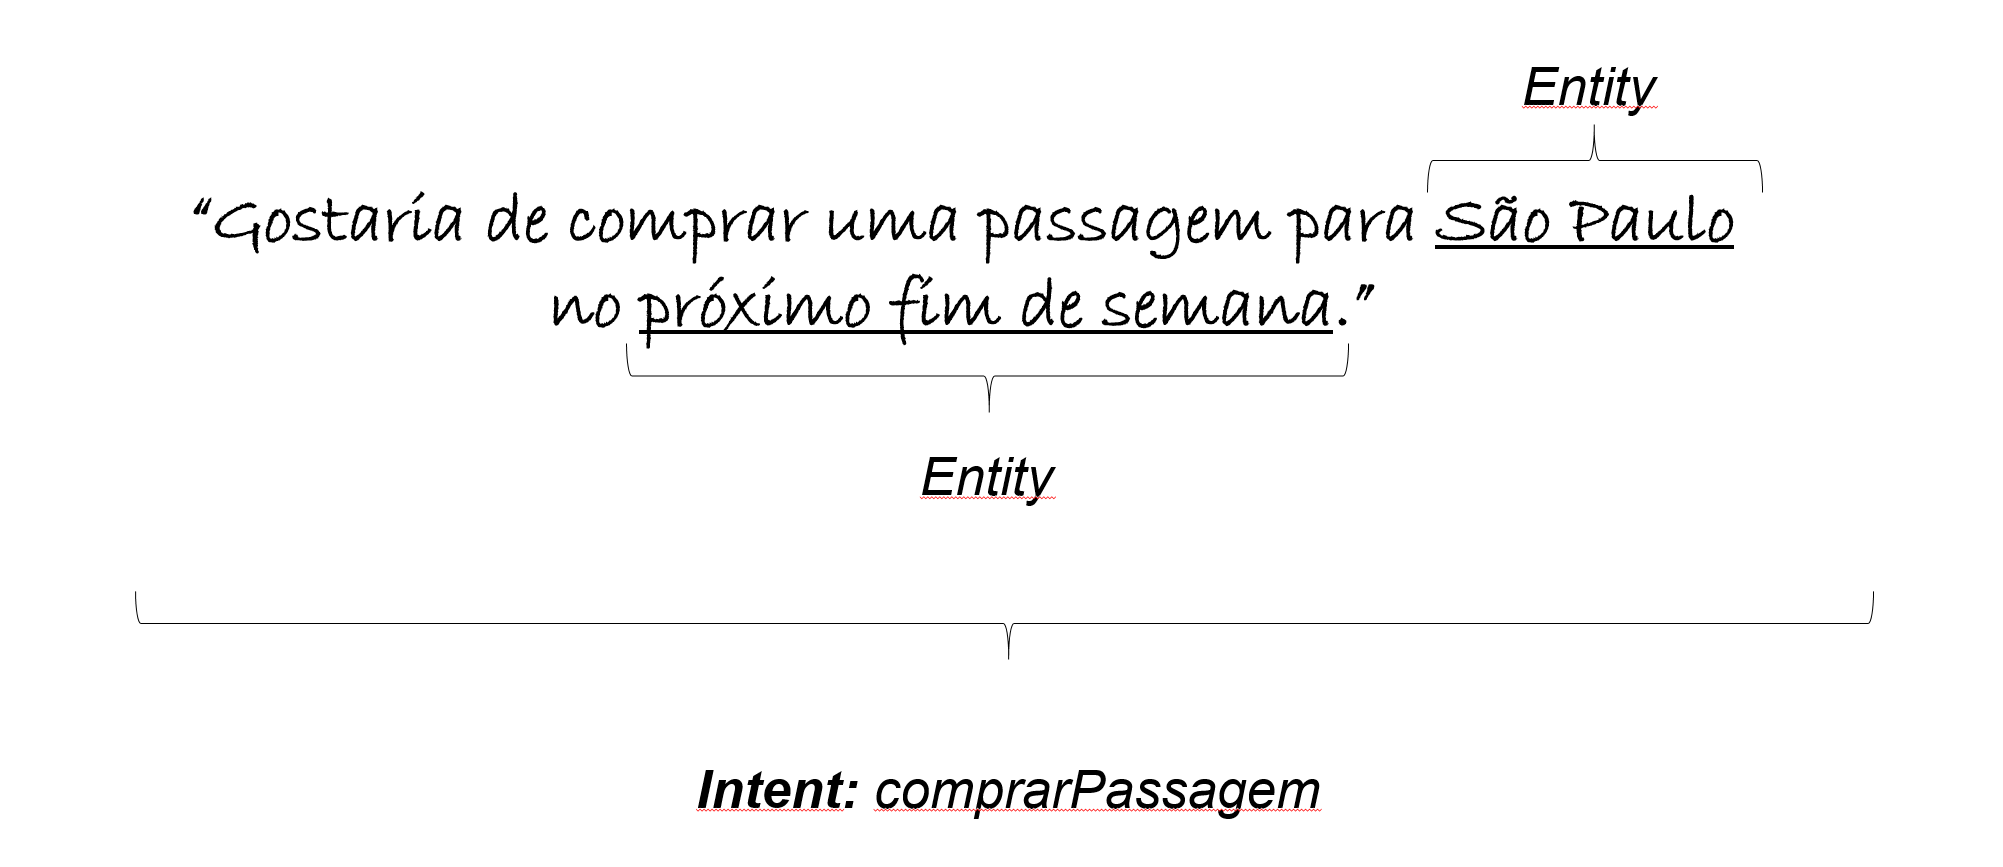
\includegraphics[width=0.95\linewidth]{images/nlp.png}
  		\caption{Interpretação de uma frase com processamento de linguagem natural}
  		\label{fig:nlp}
  	\end{center}
  \end{figure}
  
  A frase tem como objetivo (\textit{intent}) comprar uma passagem. Na frase, é possível identificar palavras que agregam para o objetivo de compra de passagem, como o destino (São Paulo) e data de partida (próximo fim de semana).
  
  \section{Chatbot baseado em regras}
  %Descrever todas as seções desse capítulo baseado nos artigos da base de artigos.
  %É um tipo de chatbot que funciona através de comandos específicos pré-definidos, tornando-os limitados às regras que ele conhece. De forma geral, os fluxos de conversa são bem definidos.
  \textit{Chatbots} baseados em regras são um tipo particular de \textit{bots} onde os fluxos de conversa são bem definidos e com opções mais limitadas de interação.
  
  A LEGO\footnote{https://www.messenger.com/t/LEGO}, fabricante de brinquedos infantis, possui um chatbot baseado em regras disponível na sua página do Messenger que é responsável por fornecer sugestões de presentes aos usuários baseado em um filtro de busca. O usuário fornece informações como localização, idade da criança e orçamento disponível e o \textit{bot} exibe as opções disponíveis.
  
  \section{Chatbots com inteligência artificial}
  Chatbots com inteligência artificial são aqueles que conseguem extrair informações de \textit{intents} e \textit{entities} de um texto enviado pelo usuário através de algoritmos de \textit{machine learning}, e também tomar decisões com base nos dados extraídos e o contexto da conversa.
  
  Em geral, os chatbots com inteligência artificial são treinados previamente para conhecer uma série de respostas para os \textit{intents} que ele irá atender. Sendo assim, ele não será capaz de responder a situações no qual ele não seja treinado.
  %Um chatbot inteligente é aquele que aprende com o tempo, ou com o treinamento. É caracterizado por tentar entender a linguagem natural de frases, em diversos contextos. Quanto mais treinado, melhor é o desempenho.
  
  \section{Uso do chatbot}
  %Escrever sobre o uso do chatbot em diferentes áreas.
  A aplicabilidade dos chatbots é, em geral, a mesma que qualquer outro sistema computacional, pois trata-se de uma interface de interação que permite execução de comandos de máquina e integração com outros tipos de sistema de software, como bancos de dados, por exemplo.
  
  O avanço no desenvolvimento das plataformas de bots, liderado principalmente pelo Facebook tornou possível a criação de chatbots que resolvem problemas reais da população, como é o caso do PrefeitoBot\cite{prefeitobot}. O PrefeitoBot é um bot para Messenger que traz informações sobre a prefeitura da cidade do Rio de Janeiro, como secretarias e horários de funcionamento. Além disso, também oferece um canal onde os usuários podem reportar ocorrências na cidade, como tombamento de árvores, alagamentos, poluição sonora, entre outras situações que o canal 1746 da cidade do Rio de Janeiro oferece atendimento.
  
  Chatbots também estão presentes no setor de varejo. As Casas Bahia lançou em 2017 o Bahianinho\footnote{https://www.facebook.com/CasasBahia/}, o chatbot da empresa responsável pelo atendimento dos consumidores através do \textit{Messenger}. Na época, sua principal função era enviar ofertas da Black Friday para os usuários, de acordo com suas preferências.
  
  No mesmo ano, o Rock in Rio criou o Roque\footnote{https://take.net/blog/take-notes/case-take-chatbot-no-rock-in-rio/}. O bot do festival interagiu com mais de 77 mil usuários, trocando cerca de 3 milhões de mensagens\footnote{https://take.net/blog/chatbots/cases-de-chatbots-famosos/} ao longo dos 7 dias de evento. Roque tirava dúvidas dos usuários, enviava notícias e prestava suporte aos participantes do festival e também aos que assistiam de casa.
  
  \section{Uso do chatbot na área médica}
  Os \textit{chatbots} podem desempenhar um papel estratégico na área médica. Em geral, por desempenhar um atendimento automatizado aos usuários que o utilizam, os \textit{chatbots} podem ser responsáveis por ser um canal disponível 24 horas por dia, podendo atender cada usuário de forma personalizada, oferecendo suporte a diversas situações da área da saúde como marcação de consultas, lembretes de medicação, dúvidas sobre doenças, etc.
  
  Hoje é possível encontrar diversos \textit{chatbots} aplicados a área médica como o \emph{HelpCare} \cite{helpcare}, que auxilia no tratamento de doenças crônicas como diabetes, colesterol alto e hipertensão arterial, e o \emph{MediBot} \cite{medibot}, que oferece informações sobre medicamentos.
  %xxxxxxxxxxxxxx
  

    \chapter{Tecnologias utilizadas na construção de chatbots}
  
  \section{Ferramentas e Frameworks}
  \subsection{Chatfuel}
  Chatfuel é o \textit{framework} mais utilizado na criação de \textit{bots}. Através de uma plataforma totalmente online, o serviço permite a criação de \textit{chatbots} através de um painel. Segundo dados da própria companhia, cerca de 46\% dos \textit{chatbots} desenvolvidos para o Facebook Messenger\footnote{Disponível em https://chatfuel.com/} são criados com a plataforma.
  
  Com o Chatfuel é possível criar \textit{bots} baseados em regras ou com inteligência baseada em palavras-chave, com treinamento feito diretamente pelo painel de administração.
  
  O plano gratuito permite até 1000 usuários assinantes e exibe uma propaganda no \textit{chatbot} indicando que ele foi desenvolvido com a ferramenta.
  
  \subsection{Botpress}
   O Botpress é um \emph{framework} \emph{open-source} de criação de bots desenvolvido em JavasScript que contém toda a infraestrutura necessária para produzir chatbot sem a necessidade de escrever muito código. Executado com o Node.js e disponível no repositório do NPM, o Botpress é focado na simplicidade e na intuitividade para o desenvolvimento de \textit{chatbots}, oferecendo um painel interativo para criação de fluxos de conversa e um simulador para testes, o que permite a construção de um \textit{chatbot} completo de forma bem mais rápida. Além disso, também é possível adicionar novas funcionalidades através da instalação de módulos.
  
   Os módulos do Botpress são componentes que não fazem parte do Core principal do \textit{framework}, mas que podem ser instalados para adicionar novas funcionalidades. Os módulos se dividem em três categorias: módulos de canais, módulos de skills e módulos funcionais.
  
  Os módulos de canais são os componentes que permitem com que o \textit{chatbot} envie e receba mensagens de uma plataforma específica, como Facebook Messenger, Telegram, etc. Para que isso aconteça, o Botpress Core implementa um mecanismo de enfileiramento que processa as mensagens que chegam e que saem, sequencialmente. Caso haja alguma falha nesse processo (um erro de envio, por exemplo) é feita uma nova tentativa de processamento da mensagem, antes de gerar um erro.
  
  Skills são componentes que podem ser incluídos nos fluxos de conversa. Dessa forma, os módulos de skills são aqueles módulos que instalam tais componentes. Um exemplo de módulo de skill, por exemplo, é o \textbf{múltipla escolha}.
  
  \begin{figure}[h!]
  	\begin{center}
  		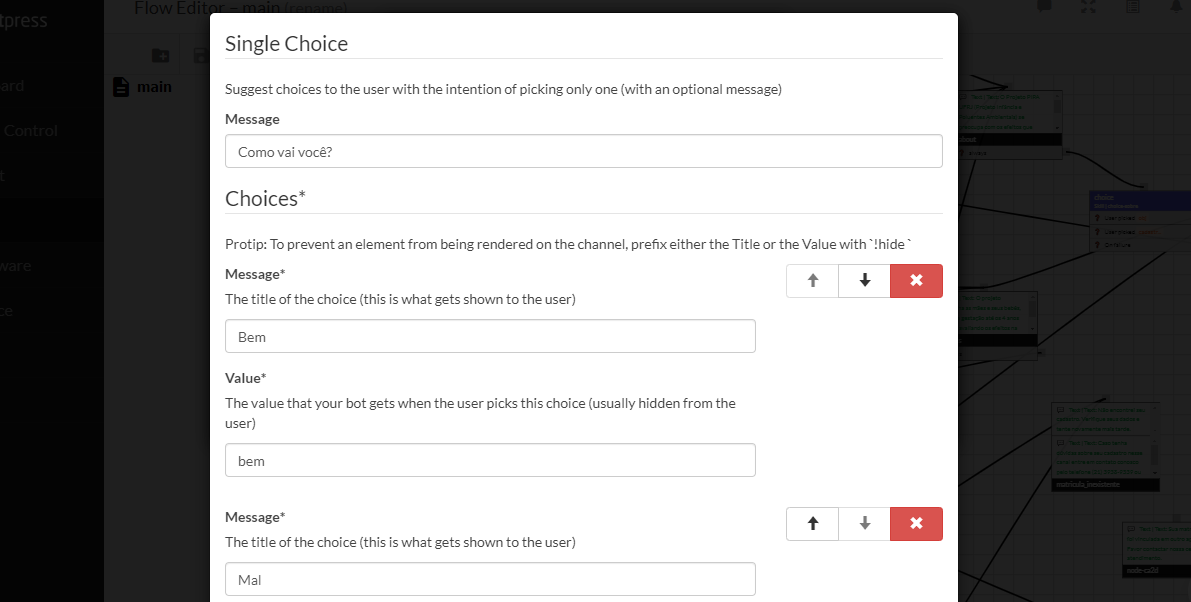
\includegraphics[width=0.95\linewidth]{images/choice.png}
  		\caption{\textit{Choice} - Componente de respostas através de opções de múltipla escolha}
  		\label{fig:choice}
  	\end{center}
  \end{figure}
  
  Diferentemente dos módulos de skill e de canais, que estendem as funcionalidades já existentes do Botpress, os módulos funcionais são aqueles que incluem funcionalidades novas. Um exemplo de módulo funcional é o HITL (Human in the loop). Com esse módulo, é possível pausar o \textit{chatbot} em conversas específicas, permitindo um humano interagir com o usuário diretamente pelo painel, como mostrado na figura \ref{fig:hitl}.
  
  \begin{figure}[h!]
  	\begin{center}
  		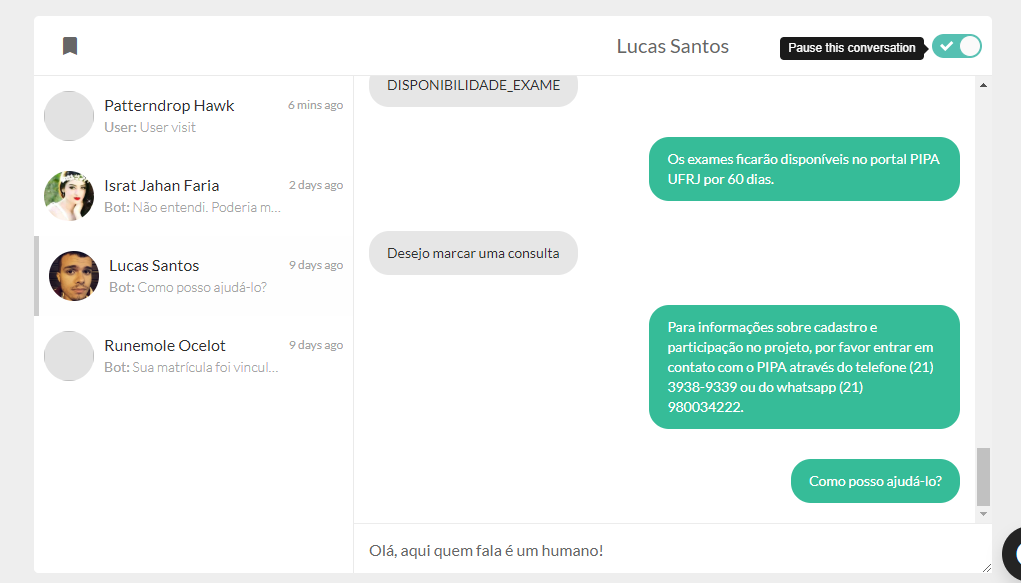
\includegraphics[width=0.95\linewidth]{images/hitl.png}
  		\caption{\textit{HITL} - Interface de troca de mensagens no painel do Botpress}
  		\label{fig:hitl}
  	\end{center}
  \end{figure}
  
  Por fim, o Botpress também permite criar \emph{actions} (ações). Essas ações são trechos de código escritos em JavaScript que, diferente dos módulos, só são executadas quando invocados por algum bloco do fluxo da conversa, como na figura \ref{fig:action}.
  
  \begin{figure}[h!]
  	\begin{center}
  		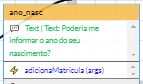
\includegraphics[width=0.35\linewidth]{images/action.png}
  		\caption{\textit{Actions} - Bloco com uma função javascript que é executada após o envio da mensagem.}
  		\label{fig:action}
  	\end{center}
  \end{figure}
  
  
  \section{Canais}
  \subsection{Facebook Messenger}
  É o aplicativo de mensagens desenvolvido originalmente para ser a plataforma de chat do Facebook. Com ele, os usuários podem se comunicar com outros usuários da plataforma através de textos, chamada de voz ou vídeo e também compartilhar diversos tipos de mídia e arquivos.% Dentre os tipos de mídia, é possível compartilhar fotos, vídeos, figurinhas, áudios e até mesmo outros formatos de arquivos em geral (acessados via download).
  
  Em 2016 o Facebook anunciou uma plataforma de bots para o Messenger que recebe constantes melhorias desde então. Hoje, é possível que usuários façam \textbf{assinaturas} para receber conteúdos diretamente dos bots que ele conversa. Por padrão, os bots apenas respondem a mensagens de usuários mas com uma assinatura é possível com que o bot proativamente envie a mensagem.
  
  %Além disso, é possível gerar QR Codes que podem ser lidos pela câmera do Facebook Messenger que levam os usuários diretamente para uma janela de conversa com o bot.
  \subsection{Telegram}
  É um aplicativo de troca de mensagens multiplataforma, podendo ser acessado através de smartphones, computadores, ou pela interface web. Assim como o Messenger, é possível compartilhar arquivos de mídia com outros usuários. Por sua infraestrutura ser baseada em nuvem, é possível acessar as mídias de uma conversa de qualquer lugar. Além disso, todos os clients do Telegram são opensource, e o serviço disponibiliza APIs para desenvolvedores criarem suas aplicações.
  
  No Telegram, bots são um tipo especial de conta que não requer um número telefônico para ser criado. Os usuários interagem enviando mensagens e comandos pela conversa ou adicionando o bot a grupos. As mensagens são armazenadas nos servidores do Telegram até que o serviço que controle o bot leia e processe as mensagens. Os bots não podem enviar mensagens diretamente para qualquer usuário; é preciso que o usuário inicie uma conversa ou que ele seja adicionado a um grupo.
  
  
  \subsection{Slack}
  Slack é uma ferramenta colaborativa que tem como objetivo reunir pessoas, informações e as ferramentas certas para desenvolver algum tipo de trabalho. É largamente usado como ferramenta de comunicação em empresas.
  
  Na plataforma, bots são um tipo de aplicativo que interage com o usuário através da conversação. Ele recebe exatamente os mesmos acessos que uma aplicação comum do Slack (inclusive, ao adicionarmos um bot, adicionamos uma integração - que é limitado pelo plano gratuito do Slack), com diferença que ele se torna um usuário como um outro qualquer do espaço colaborativo. É possível mencioná-lo em conversas, é possível mandar mensagens diretas, enviar arquivos e adicionar em grupos. Além disso, bots tem permissões para abrir uma nova conversa com algum usuário caso seja programado para isso.
  %\subsection{WhatsApp}
  
  \section{Provedores de inteligência artificial e NLP}
  \subsection{Wit.ai}
  Wit.ai é um provedor de inteligencia artificial e processamento de linguagem natural gratuito criado pelo Facebook para ser integrado a diversos tipos de aplicações de software como aplicativos, wearables e bots\footnote{https://wit.ai/}. Suporta cerca de 50 linguagens diferentes.
  \subsection{IBM Watson}
  IBM Watson é uma suíte completa de ferramentas voltadas para inteligência artificial. Desenvolvida pela IBM, tem como principal destaque a precisão na detecção de intents mesmo com uma base de treino pequena. Com o Watson Assistant é possível desenvolver gratuitamente um \textit{chatbot} sendo limitado a 10.000 chamadas de API por mês\footnote{https://www.ibm.com/watson/how-to-build-a-chatbot}.
  \subsection{LUIS.ai}
  É um serviço baseado em machine learning criado pela Microsoft focado em fornecer processamento de linguagem natural para bots, apps e dispositivos IoT. Desenhado para reconhecer informações de valor em mensagens de texto, o LUIS.ai é capaz de se integrar a outras ferramentas que compõem a suíte de aplicativos do Azure, como o Azure Bot Service\footnote{https://www.luis.ai/home}. Atualmente suporta cerca de 13 linguagens diferentes\footnote{https://docs.microsoft.com/pt-br/azure/cognitive-services/luis/luis-language-support}.
  %\section{outras coisas????}
  
  %Colocar tudo que você usou. Veja como a Andrea fez.
  
  
    \chapter{Desenvolvimento do chatbot}
  
  \section{Motivação}
  
  \subsection{Contexto: o projeto PIPA UFRJ}
  
  O Projeto Infância e Poluentes Ambientais – PIPA UFRJ é um estudo epidemiológico denominado "Estudo longitudinal dos efeitos da exposição a poluentes ambientais sobre a saúde infantil - Coorte dos bebês". Este estudo tem como proposta fornecer informação que permita a investigação e análise dos efeitos dos poluentes ambientais especificamente: metais (chumbo, mercúrio, cádmio e arsênio), agrotóxicos e plastificantes, sobre o desenvolvimento das crianças, desde o período de gestação e nascimento, até os 4 anos de idade. 
  
  Em 2017 iniciou-se a fase de estudo piloto do projeto, avaliando a exposição da mãe e seu filho até os 6 meses de idade, além de suas informações sociodemográficas. Nessa fase as metodologias e estratégias propostas estão sendo testadas e validadas, a fim de aprimorar o estudo. Como resultado desse projeto, vai ser possível propor medidas preventivas e de controle, o que melhoraria a qualidade de vida da população.
  
  O projeto é promovido pela Universidade Federal do Rio de Janeiro (UFRJ) realizado pela Maternidade Escola, pela Faculdade de Medicina e pelo Instituto de Estudos em Saúde Coletiva (IESC/UFRJ) e conta com diversos parceiros como a Fundação Oswaldo Cruz (FIOCRUZ) e o Centro de Estudos da Saúde do Trabalhador e Ecologia Humana (CESTEH).
  
  \subsection{Tecnologias utilizadas no PIPABOT}
  \subsubsection{Node.JS}
  Node.js é um interpretador de código JavaScript construído sobre a máquina virtual Javascript V8 do Google, cujo foco é executar aplicações baseadas em rede no lado do servidor.
  
  %Historicamente a linguagem JavaScript é conhecida por ser a linguagem padrão executada por \emph{browsers} no lado do cliente mas com a rápida evolução da web nos últimos anos, os motores de execução da linguagem receberam diversas melhorias, tornando viável a execução de códigos que vão além de manipulação de HTML.
  
  A principal característica que diferencia o Node.js de outras tecnologias \emph{server-side} como o PHP, é o fato de sua execução ser \emph{single-thread}, ou seja, apenas uma thread é responsável por executar a aplicação, enquanto que outras linguagens a execução é \emph{multi-thread}.
  
  Os modelos tradicionais de aplicações web criam novas threads para cada requisição recebida, o que demanda recursos computacionais como memória RAM, por exemplo. Como esses recursos são limitados, haverá um número máximo de threads que poderão ser criadas até que os recursos sejam liberados novamente.
  
  \begin{figure}[h!]
  	\begin{center}
  		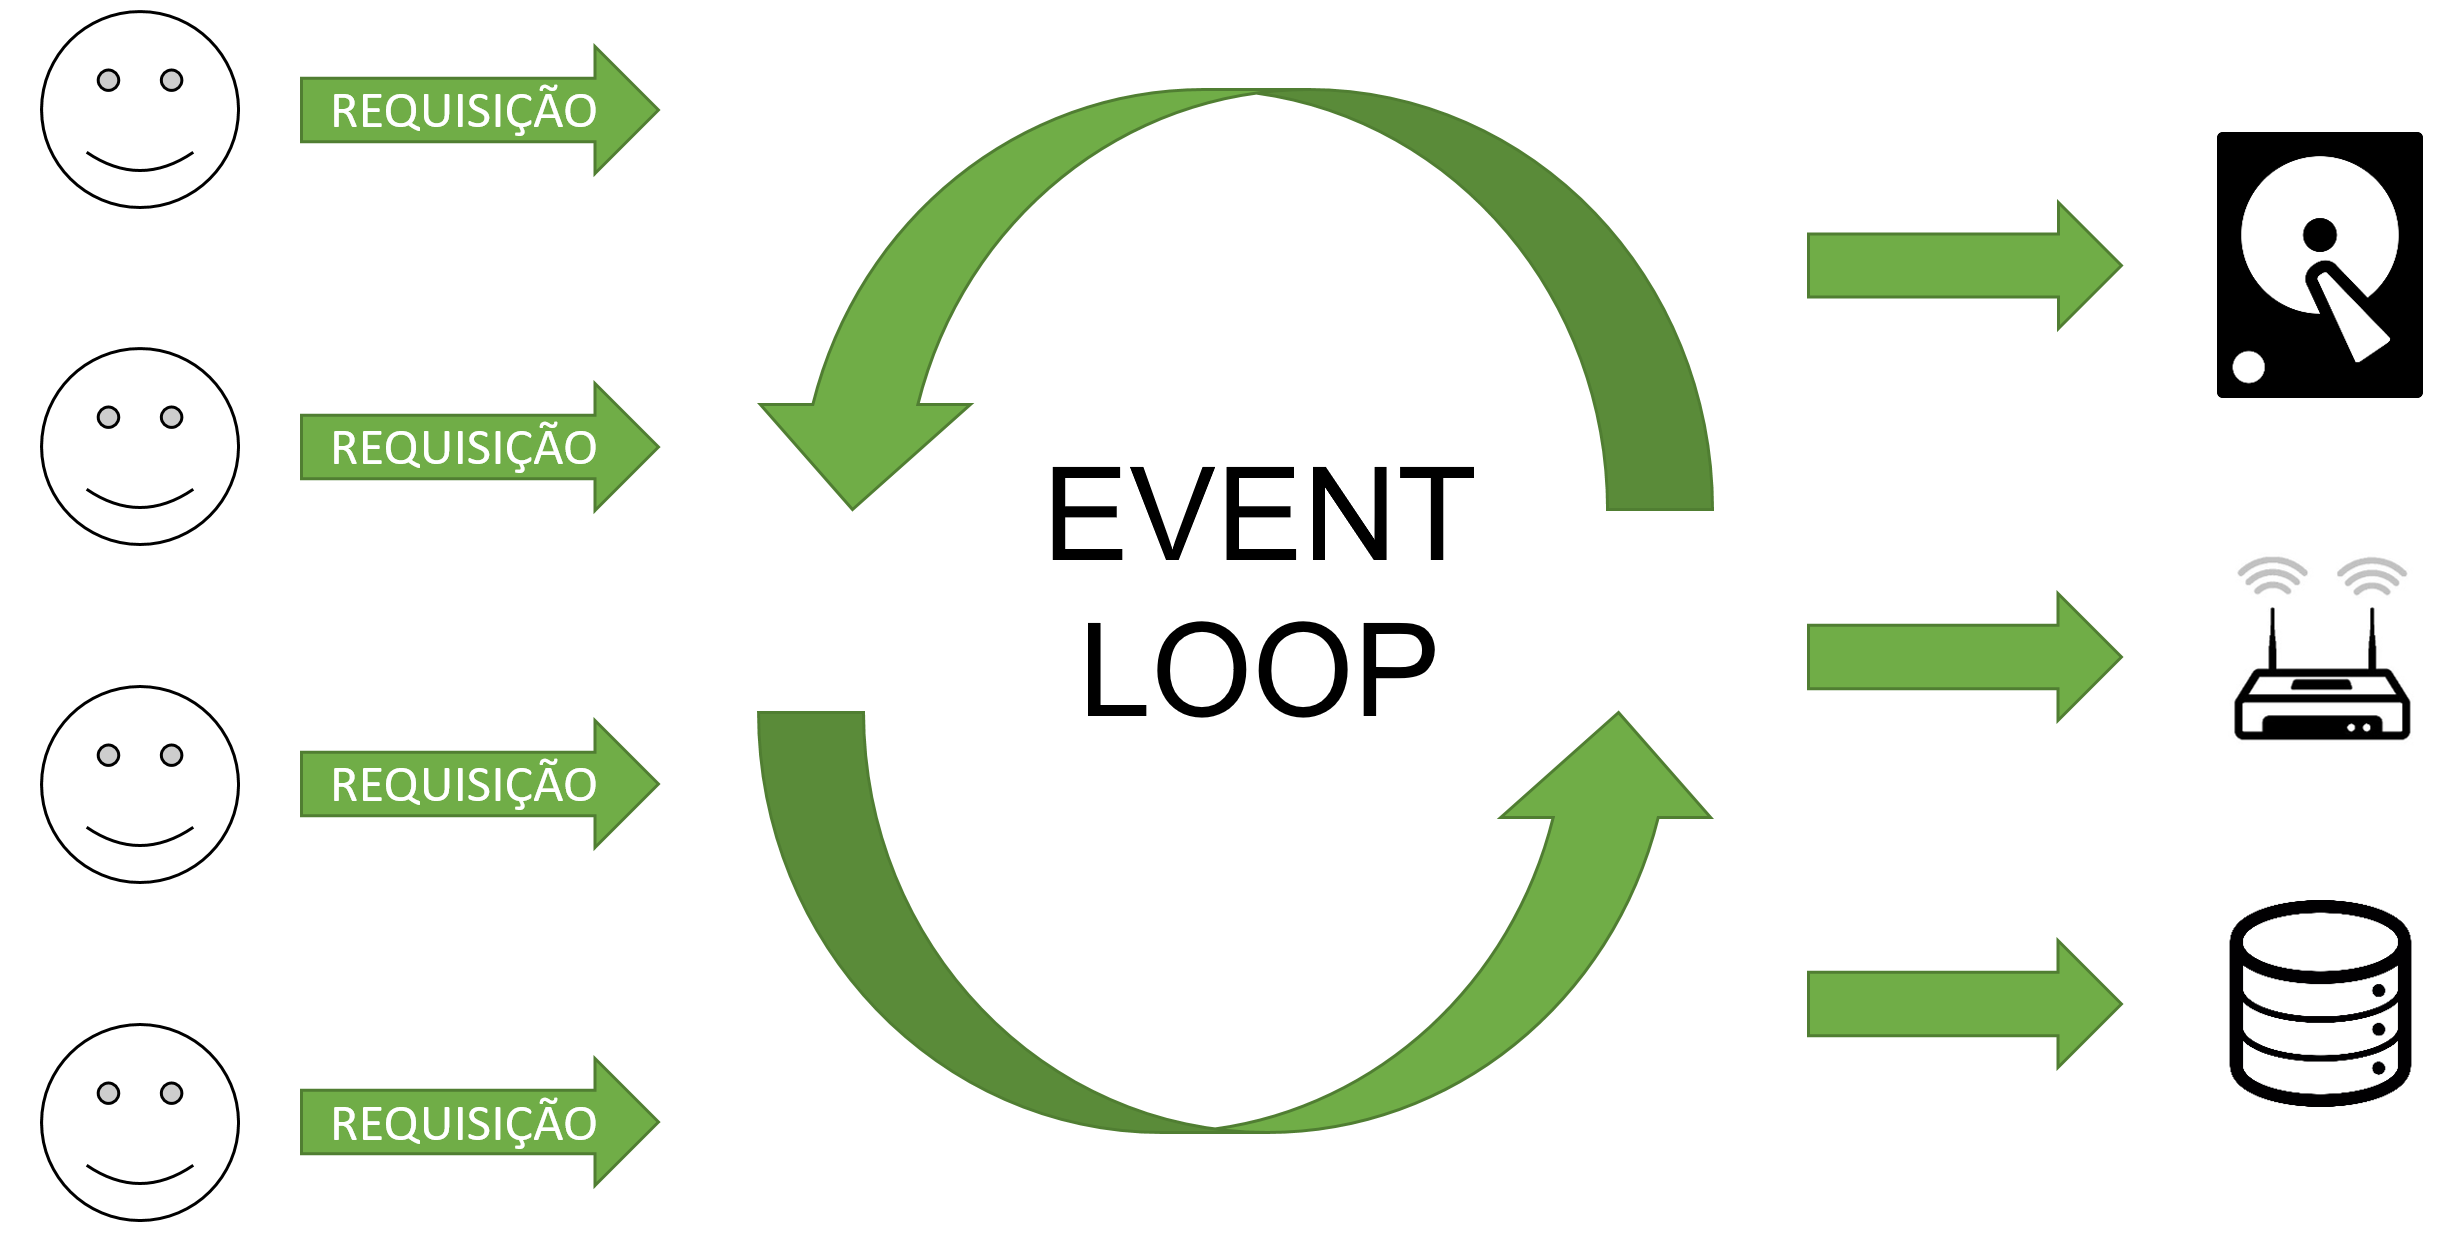
\includegraphics[width=1\linewidth]{images/node_thread.png}
  		\caption{Arquitetura do NodeJS}
  		\label{fig:node}
  	\end{center}
  \end{figure}
    
  No Node.js as requisições são tratadas por uma única thread, chamada de Event Loop. A thread é executada esperando eventos para tratar. Quando chega uma nova requisição, um evento é criado.
  
  Para tratar a concorrência de requisições, o Node.js faz uso de chamadas de E/S não-bloqueantes. Assim, a sua única thread não fica esperando as demais chamadas já realizadas serem concluídas para continuar sua execução.
  
  Graças a sua arquitetura, o Node.js consegue tratar um número maior de requisições concorrentes do que uma aplicação no modelo tradicional, se mostrando como uma das plataformas mais escaláveis da atualidade.
  
  \subsubsection{NPM}
  Node Package Manager, ou NPM, é o gerenciador de pacotes do Node.js. Nele é possível encontrar componentes open-source que agilizam o desenvolvimento de aplicações como conectores para bancos de dados, servidores web completos, entre outros. Além disso, o NPM também faz o gerenciamento de dependências de um projeto.
  
  Ao instalar um componente com o comando \emph{npm install <componente>} em um projeto do Node.js, o utilitário adiciona o pacote e a versão utilizada e suas dependências em um arquivo chamado package.json;  
  Desse modo é possível restaurar todas as dependências do projeto, caso seja necessário.
  
  \subsubsection{Git}
  Git é um sistema de versionamento de código distribuído que possui diversas ferramentas úteis para o desenvolvimento de um sistema. Sua escolha se deu pelo fato de ser open source, e por permitir criar ramificações (branches) de código a partir de um ponto do desenvolvimento, permitindo criar diferentes versões independentes entre os ramos\footnote{https://git-scm.com/about}. Através do uso de branches, foi criado um Git Flow para o PipaBot, como na figura \ref{fig:gitflow}.
  
  \begin{figure}[h!]
  	\begin{center}
  		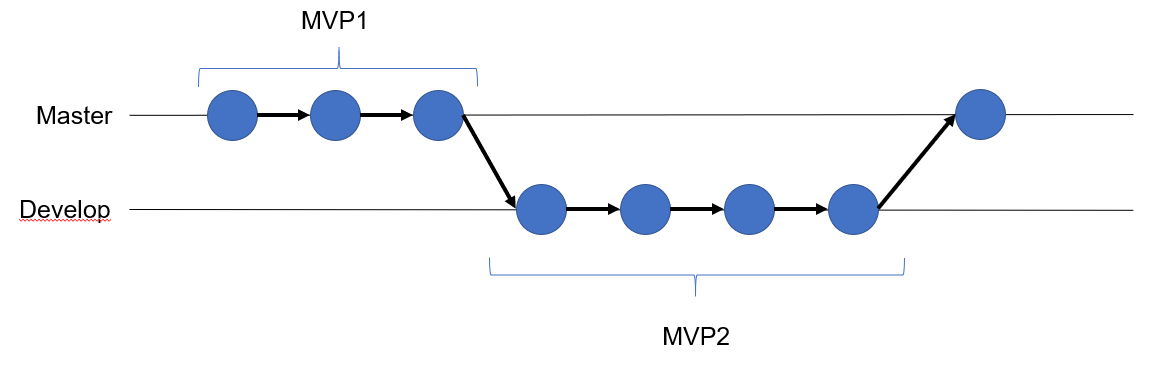
\includegraphics[width=1\linewidth]{images/git_flow.png}
  		\caption{PipaBot - Organização do versionamento do código}
  		\label{fig:gitflow}
  	\end{center}
  \end{figure}
  
  Após o desenvolvimento da primeira versão do PipaBot, foi criada uma nova branch de desenvolvimento da próxima interação do ciclo Construir-Medir-Aprender. Isso foi feito para que a branch principal do repositório (master) possuísse um produto pronto para ser executado. Ao término da segunda versão do MVP, foi feito um merge da branch de desenvolvimento com a master.
  
  

  \section{Ambientes de desenvolvimento} % trocar a ordem com arquitetura?
  O PipaBot foi desenvolvido em uma estrutura formada por dois ambientes: um ambiente de desenvolvimento e um ambiente de homologação.
  
  O ambiente de desenvolvimento é executado no próprio computador onde as implementações são feitas e é acessível apenas localmente. É composto de um servidor HTTP do Botpress, que gera uma instância do PipaBot, tornando possível testar funcionalidades através de um chat na URL \url{http://localhost:3000/s/chat}.
  
  O ambiente de homologação é composto por dois servidores HTTP e um servidor de banco de dados MySQL, todos localizados na nuvem e recebem as versões incrementais do \textit{bot} a cada ajuste funcional, para que sejam testadas e validadas pelos \textit{stakeholders}.
  
  Um dos servidores HTTP é o Botpress, contendo a última release do ambiente de desenvolvimento. O outro servidor HTTP executa uma instância do Wordpress, para que seja permitido simular o Portal do PIPA e validar a versão web do PipaBot. O servidor MySQL é utilizado pelo Wordpress para armazenar os dados dos usuários.
  
  \section{A solução}
  
  \subsection{Arquitetura}
  A arquitetura do PipaBot é composta por duas camadas, o \textit{front-end} e o \textit{back-end}. O \textit{front-end} é toda a interface utilizada pelo usuário para interagir com o bot (comumente chamado de canais): o portal do PIPA através da versão web, ou pelo aplicativo do Messenger em dispositivos mobile ou PC. Enquanto o \textit{back-end} é onde se encontra o processamento do \textit{bot}. É nele onde as mensagens são classificadas e as respostas, escolhidas. Além disso, o back-end também é responsável pela integração dos dados dos pacientes do Portal do PIPA com o \textit{bot}. O esquema detalhado da arquitetura pode ser visto na figura \ref{fig:arquitetura}.
  
	  \begin{figure}[h!]
	  	\begin{center}
		  	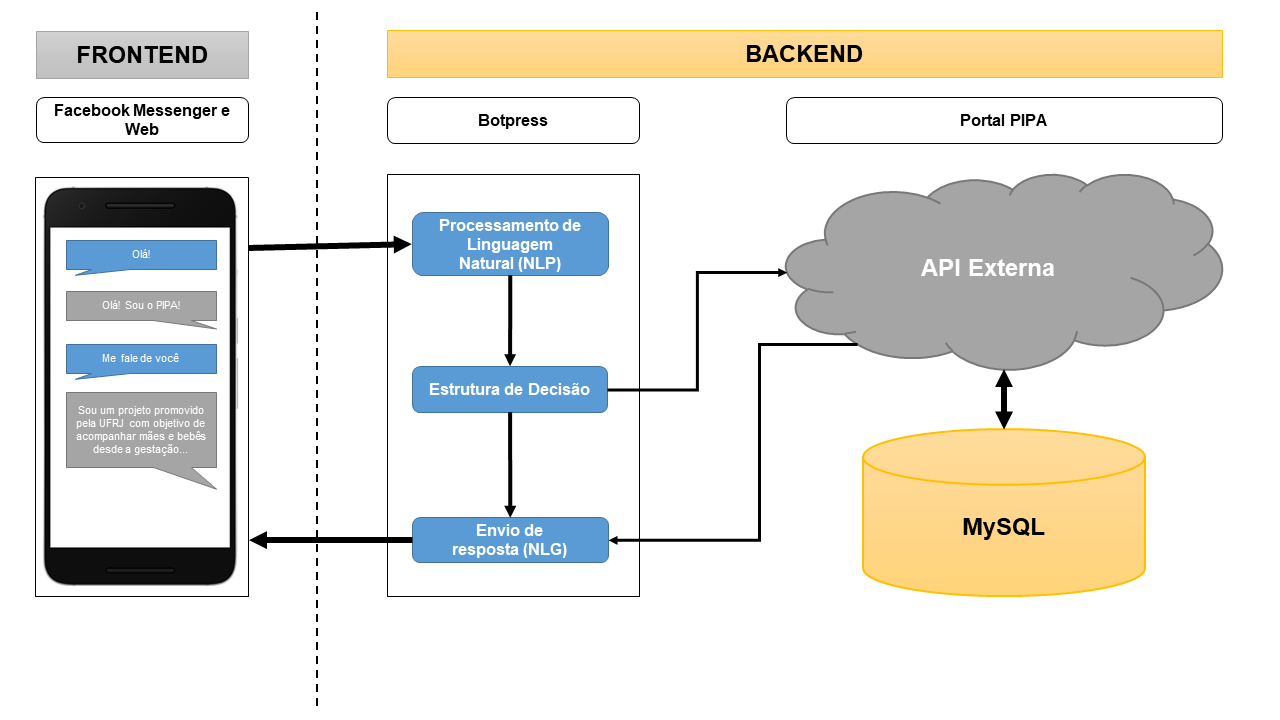
\includegraphics[width=1\linewidth]{images/arquitetura-pipabot.png}
			\caption{Arquitetura do PipaBot}
			\label{fig:arquitetura}
	  	\end{center}
	  \end{figure}
  
  Como framework de criação de bots, foi escolhido o \textbf{\textit{Botpress}}, por possuir, em uma única solução, funções como processamento de linguagem natural, criador de fluxos de conversa, estruturas de decisão (permitindo a criação de chatbots baseados em regras ou em inteligência artificial, através de classificação de intents) e suportar diversos canais de comunicação para um mesmo \textit{bot}, além de ser uma estrutura onde todo o código fica sob domínio do administrador do \textit{bot}, o que é importante principalmente para implementações de funcionalidades específicas do \textit{PipaBot} como o acesso à base de usuários, por exemplo.
  
  Para integrar o PipaBot ao Portal do PIPA, que é desenvolvido utilizando o sistema de gestão de conteúdo Wordpress (construído em PHP e MySQL), foi utilizada a própria API REST do Wordpress. Essa API implementa endpoints que permitem acessar o CRUD (\textit{Create}, \textit{Read}, \textit{Update} e \textit{Delete} - Operações de leitura e escrita de dados do sistema) de diversas tabelas que guardam o conteúdo do Portal no banco de dados, inclusive de usuários. Contudo, por padrão, as rotas de leitura de usuários apenas retornam usuários que já fizeram alguma publicação no Portal, o que não era o caso dos pacientes, que nem possuem permissão de executar tal ação. Então, foram criados três novos \textit{endpoints}, que só podem ser acessado através de autenticação através da tecnologia JWT (\textit{JSON Web Token}), que utiliza o perfil de um usuário administrador do Portal. Esses \textit{endpoints} são responsáveis por (I) verificar se um usuário existe através do seu CPF e ano de nascimento, e (II) por adicionar um identificador do usuário do \textit{chatbot} no cadastro do Portal e (III) por verificar se um usuário do bot está atrelado a um cadastro de paciente no Portal - através do identificador cadastrado no \textit{endpoint} II. 
  
  Para tornar a instalação dos recursos do PipaBot mais ágil e manutenível, todos as implementações dos \textit{endpoints} foram encapsulados em um arquivo PHP que é reconhecido pela instalação do Wordpress como um plugin, que pode ser ativado ou desativado a qualquer momento através do painel do administrativo do Portal.
  
  \subsection{Modelos}
  	\begin{center}
  		\begin{tabular}{ | m{0.2\linewidth} | m{0.26\linewidth} | m{0.26\linewidth} | m{0.26\linewidth} | } 
  			\hline
  			\textbf{Identificação} & \multicolumn{3}{l|}{RF01}\\ 
  			\hline
  			\textbf{Casos de Uso Relacionados} & \multicolumn{3}{l|}{TESTE}\\ 
  			\hline
  			\textbf{Descrição} & \multicolumn{3}{l|}{Lorem ipsum damet...}\\ 
  			\hline
  			\textbf{Prioridade} & [ ] Essencial & [ ] Importante & [ ] Desejável \\
  			\hline
  		\end{tabular}
  	\end{center}
  
%	-  	Mapeamento de casos de uso
	
%	-	Diagrama de Atividades
	
%	-	Especificação dos Requisitos
	\begin{figure}[h!]
	 	\begin{center}
	 		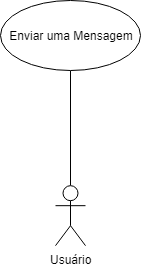
\includegraphics[scale=0.6]{images/UC_Usuario.png}
	 		\caption{Casos de Uso do Usuário}
	 		\label{fig:ucusuario}
	 	\end{center}
	\end{figure}

	\begin{figure}[h!]
		\begin{center}
			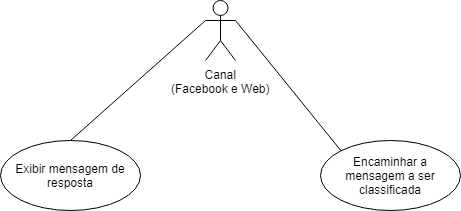
\includegraphics[width=12cm]{images/UC_Canal.png}
			\caption{Casos de Uso do Canal (Messenger e Web)}
			\label{fig:uccanal}
		\end{center}
	\end{figure}
	
	\begin{figure}[h!]
		\begin{center}
			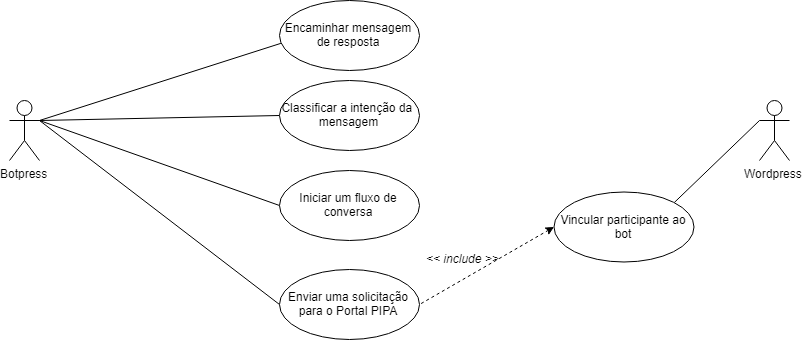
\includegraphics[width=1\linewidth]{images/UC_Botpress_Wordpress.png}
			\caption{Casos de Uso do Bot}
			\label{fig:ucbot}
		\end{center}
	\end{figure}
  \FloatBarrier
  \subsection{MVP 1}
  Tendo como principal problema a falta de engajamento das mães com o projeto e buscando criar um novo canal de informação sobre o PIPA, o PipaBot teve a sua primeira versão orientada a regras. Para garantir que o usuário navegasse através dos fluxos de conversa, o \textit{bot} exibia botões, de modo que o usuário não desviasse a conversa para um outro assunto no meio de um fluxo. Essa versão era capaz de dar informações sobre o funcionamento e objetivo do projeto, e vincular usuários a um cadastro no Portal do PIPA.
  
  O principal objetivo da primeira versão era apresentar aos pesquisadores do projeto o que um \textit{chatbot} poderia ser capaz de fazer, demonstrando integrações com o sistema do PIPA e elementos de interação, visando novas ideias para a versão seguinte.
  \subsection{MVP 2}
  A segunda versão do PipaBot trouxe diversas melhorias. Foram criados diálogos exclusivos para pacientes do projeto como informações sobre consultas e exames além de ter também o treinamento para diversos \textit{intents}, que eram reconhecidos através da tecnologia de NLP do Botpress. Cada \textit{intent} levava a um fluxo de conversa diferente cuja interação poderia ser feita não somente por botões, mas textualmente, dando mais naturalidade ao diálogo.
  \subsection{Avaliação do produto}
  %falar do TAM e mostrar os resultados. 
  Para avaliar o PipaBot foi utilizado o modelo TAM (\textit{Technology Acceptance Model})\cite{tam_davis} que procura determinar os aspectos de utilidade e facilidade de uso de tecnologias. Para isso, o TAM se baseia nos conceitos de \textbf{percepção de utilidade} e \textbf{percepção de facilidade de uso}, métricas que avaliam, respectivamente, o quanto o usuário acredita que a tecnologia possa melhorar seu desempenho e o quanto ele acredita que, ao utilizar a tecnologia, ele possa ficar livre de esforço físico e mental.
  
  Para elaboração do TAM, foi utilizado o paradigma GQM (\textit{Goal/Question/Metric}), ilustrado na figura \ref{fig:gqm}, que consiste em descrever os objetivos (\textit{Goals}), a partir dos objetivos elaborar um conjunto de questões (\textit{Questions}) e, então, métricas (\textit{metrics}) para medir as respostas. Os objetivos do PipaBot estão definidos nas tabelas abaixo.
  
  \begin{figure}[h!]
  	\begin{center}
  		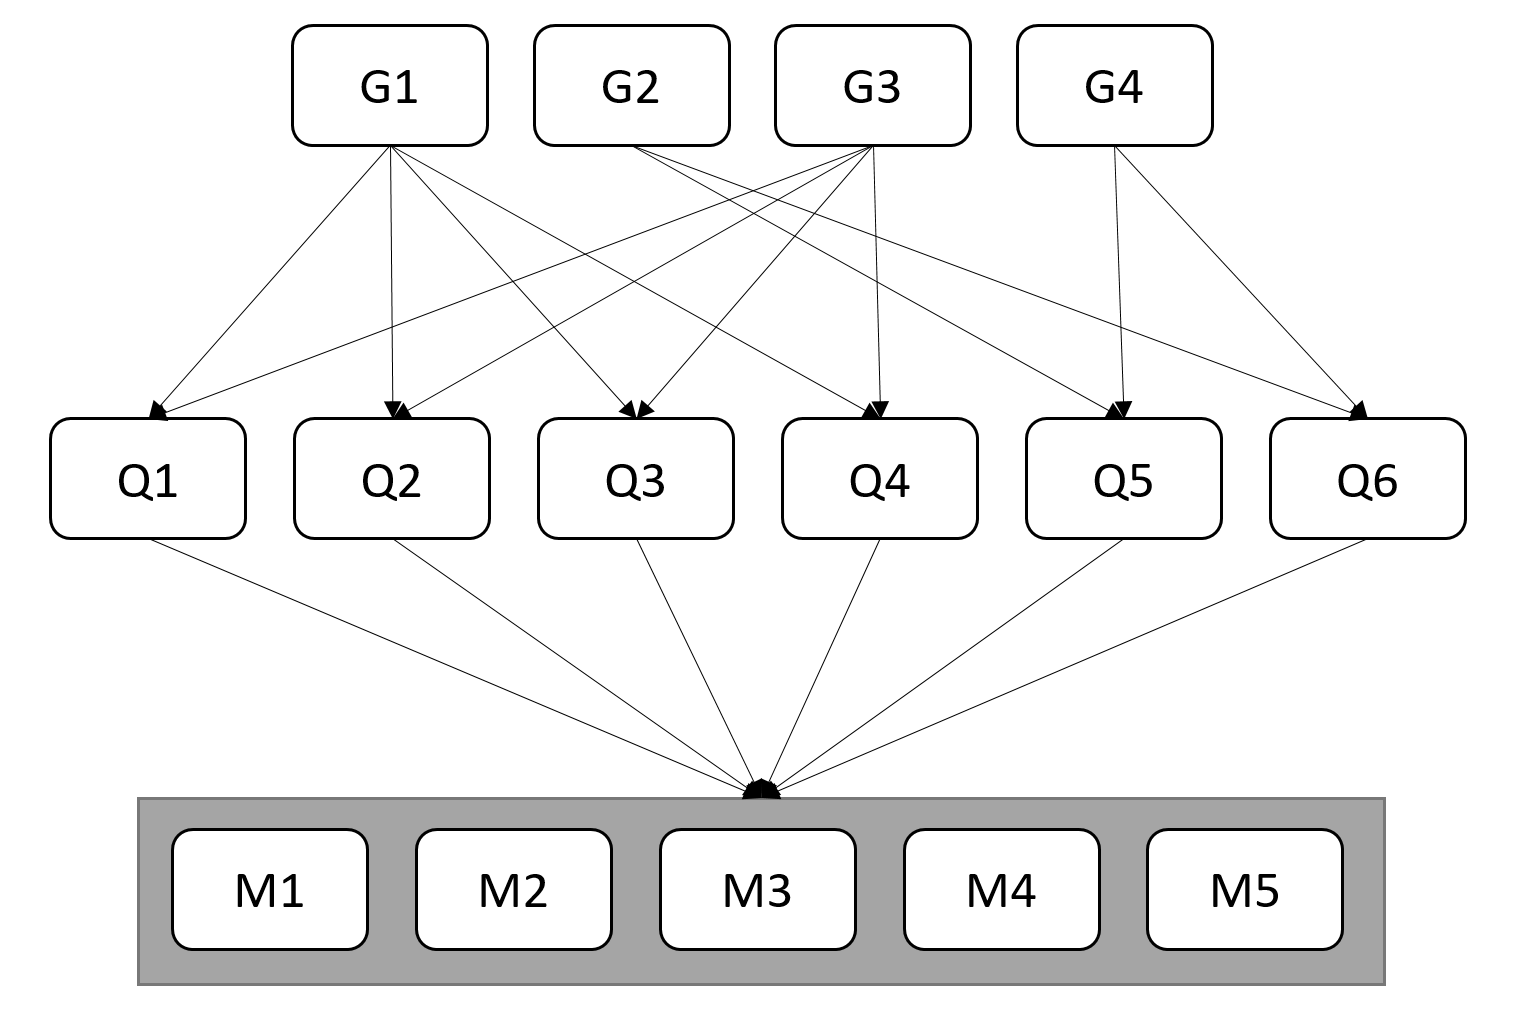
\includegraphics[width=1\linewidth]{images/gqm.png}
  		\caption{Organização do Paradigma GQM aplicado ao PipaBot}
  		\label{fig:gqm}
  	\end{center}
  \end{figure}
  
  \begin{center}
  	\begin{table}[h!]
  		\begin{tabular}{ | m{0.35\linewidth} | m{0.65\linewidth} | } 
  			\hline
  			\textbf{Analisar} & O PipaBot (chatbot do PIPA) \\ 
  			\hline
  			\textbf{Com o propósito de} & Caracterizar \\ 
  			\hline
  			\textbf{Com respeito a} & Facilidade de uso (número de mensagens e tempo de resposta) \\ 
  			\hline
  			\textbf{Sob o ponto de vista de} & Profissionais de computação \\
  			\hline
  			\textbf{No contexto de} & Profissionais de computação (estudantes de graduação e pós graduação) realizando tarefas de busca de informação no PipaBot. \\
  			\hline
  		\end{tabular}
  	  \caption{GQM - Objetivo 1}
  	  \label{tab:obj1}  	  
  	\end{table}
  \end{center}

	\begin{center}
		\begin{table}[h!]
			\begin{tabular}{ | m{0.35\linewidth} | m{0.65\linewidth} | } 
				\hline
				\textbf{Analisar} & O PipaBot (chatbot do PIPA) \\ 
				\hline
				\textbf{Com o propósito de} & Compreender \\ 
				\hline
				\textbf{Com respeito a} & Utilidade (pertinência e adequação do conteúdo da resposta) \\ 
				\hline
				\textbf{Sob o ponto de vista de} & Profissionais de computação \\
				\hline
				\textbf{No contexto de} & Estudantes de graduação e pós-graduação do sexo feminino realizando tarefas de busca de informação no PipaBot. \\
				\hline
			\end{tabular}
			\caption{GQM - Objetivo 2}
			\label{tab:obj2}
		\end{table}
	\end{center}
	
	\begin{center}
		\begin{table}[h!]
			\begin{tabular}{ | m{0.35\linewidth} | m{0.65\linewidth} | } 
				\hline
				\textbf{Analisar} & O PipaBot (chatbot do PIPA) \\ 
				\hline
				\textbf{Com o propósito de} & Caracterizar \\ 
				\hline
				\textbf{Com respeito a} & Facilidade de uso (número de mensagens e tempo de resposta) \\ 
				\hline
				\textbf{Sob o ponto de vista de} & Profissionais de saúde \\
				\hline
				\textbf{No contexto de} & Profissionais de saúde (estudantes de pós-graduação) realizando tarefas de busca de informação no PipaBot. \\
				\hline
			\end{tabular}
			\caption{GQM - Objetivo 3}
			\label{tab:obj3}
		\end{table}
	\end{center}

	\begin{center}
		\begin{table}[h!]
			\begin{tabular}{ | m{0.35\linewidth} | m{0.65\linewidth} | } 
				\hline
				\textbf{Analisar} & O PipaBot (chatbot do PIPA) \\ 
				\hline
				\textbf{Com o propósito de} & Compreender \\ 
				\hline
				\textbf{Com respeito a} & Utilidade (pertinência, adequação e utilidade do conteúdo da resposta) \\ 
				\hline
				\textbf{Sob o ponto de vista de} & Profissionais de saúde \\
				\hline
				\textbf{No contexto de} & Estudantes do sexo feminino de pós-graduação na área da saúde realizando tarefas de busca de informação no PipaBot. \\
				\hline
			\end{tabular}
			\caption{GQM - Objetivo 4}
			\label{tab:obj4}
		\end{table}
	\end{center}

	Foi elaborado um conjunto de 6 questões abordando os objetivos G1, G2, G3 e G4, visando capturar a percepção de facilidade de uso e utilidade na visão dos usuários. Para medir esses dados foi utilizada a escala \textit{Likert}, no qual os participantes especificam seu nível de concordância com uma afirmação. As questões e métricas estão exibidas nas tabelas \ref{tab:questoes} e \ref{tab:metricas} respectivamente. Junto as métricas foi disponibilizado um espaço para que os participantes pudessem expressar seus comentários sobre cada questão.
	
	\begin{center}
		\begin{table}[h!]
			\centering
			\begin{tabular}{ | m{0.05\linewidth} | m{0.95\linewidth} | } 
				\hline
				\textbf{Q1} & O PipaBot é fácil de usar \\ 
				\hline
				\textbf{Q2} & O PipaBot responde rapidamente aos meus questionamentos \\ 
				\hline
				\textbf{Q3} & Eu posso obter a informação que desejo com poucas perguntas \\ 
				\hline
				\textbf{Q4} & Os elementos de navegação (menus e botões) do PipaBot facilitam a interação ao longo da conversa \\
				\hline
				\textbf{Q5} & O PipaBot fornece respostas pertinentes aos meus questionamentos \\
				\hline
				\textbf{Q6} & O PipaBot fornece respostas adequadas aos meus questionamentos \\
				\hline
			\end{tabular}
			\caption{GQM - Questões para avaliação de grau de concordância}
			\label{tab:questoes}
		\end{table}
	\end{center}

	\begin{center}
		\begin{table}[h!]
			\centering
			\begin{tabular}{ | m{0.05\linewidth} | m{0.3\linewidth} | } 
				\hline
				\textbf{M1} & Concordo Totalmente \\ 
				\hline
				\textbf{M2} & Concordo Parcialmente \\ 
				\hline
				\textbf{M3} & Indiferente \\ 
				\hline
				\textbf{M4} & Discordo Parcialmente \\
				\hline
				\textbf{M5} & Discordo Totalmente \\
				\hline
			\end{tabular}
			\caption{GQM - Métricas}
			\label{tab:metricas}
		\end{table}
	\end{center}

	...



    \chapter{Conclusão}
  
  \section{Contribuições}
  
  \section{Limitações}

  \section{Trabalhos futuros}
  
  \section{Considerações finais}

  \backmatter
  \bibliographystyle{coppe-unsrt}
  \bibliography{example}

  \appendix
  \chapter{Algumas Demonstrações}
\end{document}
%% 
%%
%% End of file `example.tex'.
